\documentclass[a4paper,12pt]{article} % Changer la taille de police c'est ici

\usepackage{framed} % Marges
\usepackage[utf8]{inputenc} %francais
\usepackage[T1]{fontenc} %francais
\usepackage[french]{babel}  %francais
\usepackage{lmodern} % Pour changer le pack de police
\usepackage{makeidx} % Index
\usepackage{graphicx} % Figures
\usepackage{wrapfig} % Figures
\usepackage{amsmath} % Maths
\usepackage{amssymb} % symboles ?
\usepackage{bclogo} % ?????
\usepackage{hyperref}
\usepackage{stmaryrd}
\usepackage[top=2cm, bottom=2cm, left=2cm, right=2cm]{geometry} %Marges

\title{Rapport Interpolaspline}

 \begin{document}


\section{Poids faible aux points aberrants}

\subsection{Introduction}
Maintenant que nos différentes détectent des points aberrants, nous voulons créer des plines prenant en compte ces points en leur donnant un poids faible et donc réduire leur impact sur le lissage.

Une des idées était d'intégrer nos poids faibles dans une méthode de lissage faisant intervenir les poids. C'est là qu'intervient la méthode LOESS.

LOESS (ou LOWESS) est une méthode de régression non paramétrique. Elle utilise la régression linéaire des moindres carrés pondérés et créé une fonction qui décrit la variation des données, point par point, en considèrant de manière plus importante les données les plus proches de ce point.

L'objectif est d'ajuster $\theta = [\theta_0, \theta_1]$ pour minimiser les moindres carrés pondérés soit : \[\sum_{i=1}^m w_i ( y_i - (\theta_0 + \theta_1 x_i))^2 \ \ \text{(1)}\]

Avec : 
\begin{itemize}
    \item[•]  $\theta_0 \ et \ \theta_1$ les paramètres inconnus dont la valeur permet d'effectuer la procédure d'ajustement  
    \item[•]  $(\theta_0 + \theta_1 x_i)$ la coordonnée en y prédite par la méthode en fonction de ces paramètres.
    \item[•]  $1 > w_i = \exp \left( - \frac{(x -x_i)^2}{2 \rho} \right)*vpoids_i > 0$ le poids Gaussien affecté par notre vecteur de poids vpoids où  $\rho$ est considéré dans notre cas comme le paramètre de lissage.
\end{itemize}

Les poids est donc donné en utilisant le calcul des moindres carrés, on a par conséquent :
\begin{itemize}
    \item[•] Plus de poids à des points près du point cible $x$ 
    \item[•] Moins de poids à des points plus loin de $x$
\end{itemize}
Autrement, si la différence $| x_i - x |$ est petite, alors le poids $w_i$ est proche de 1, et, si dans le cas contraire, elle est grande, alors $w_i$ est proche de 0. 
Notre modèle après la méthode est ajusté, ne retenant que le point du modèle qui est proche du point cible. La procédure se répète pour chaque point par ordre croissant des abscisses.


\subsection{Exemple}

\begin{figure}[htp]
    \centering
    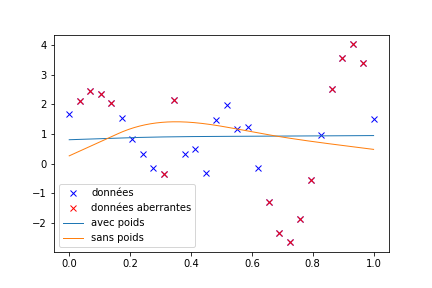
\includegraphics[width=10cm]{IMG_Tache5b_nonunif}
    \caption{Exemple de résultat }
    \label{fig:exemple}
\end{figure}

Dans cet exemple, nous avons en rouge une spline de lissage et en bleu une autre spline de lissage utilisant la méthode LOESS.  Nous avons également les valeurs initiales de l'échantillon en rouge et celle ajustées en bleu. On remarque que la méthode LOESS considère moins les valeurs pouvant être considérées comme aberrantes ou bruitées.



\subsection{Procédure}

Partons de l'expression (1) avec  x et y  des vecteurs de taille m. Appelons cette expression S en fonction de $\theta$, nous avons :
\[S(\theta) = \sum_{i=1}^m w_i \left( y_i - (\theta_0 + \theta_1 x_i) \right)^2\]

\[\frac{\partial S}{\partial \theta_0} = -2 \sum_{i=1}^m w_i \left( y_i - (\theta_0 + \theta_1 x_i) \right) \]

\[ \frac{\partial S}{\partial \theta_1} = -2 \sum_{i=1}^m w_i \left( y_i - (\theta_0 + \theta_1 x_i) \right) x_i \]


Puis :

\[\frac{\partial S}{\partial \theta_0} = \sum_{i=1}^m w_i \left( y_i - (\theta_0 + \theta_1 x_i) \right)  = 0\]

\[ \iff \sum_{i=1}^m w_i  \theta_0 + \sum_{i=1}^m w_i  \theta_1 x_i  = \sum_{i=1}^m w_i y_i  \ \ \ \text{Eq. (1)}\]

\[\frac{\partial S}{\partial \theta_1} = \sum_{i=1}^m w_i \left( y_i - (\theta_0 + \theta_1 x_i) \right) x_i  = 0\] 

\[\iff \sum_{i=1}^m w_i  \theta_0 + \sum_{i=1}^m w_i  \theta_1 x_i x_i  = \sum_{i=1}^m w_i y_i  x_i \ \ \ \text{Eq. (2)}\]


En écrivant les équations  Eq. (1) et Eq. (2) sous forme de matrice $\mathbf{A \theta = b}$ nous obtenons :



    \[\begin{bmatrix} \sum w_i & \sum w_i x_i \\ \sum w_i x_i & \sum w_i x_i x_i \end{bmatrix}  \begin{bmatrix} \theta_0 \\ \theta_1 \end{bmatrix}   = \begin{bmatrix}  \sum w_i y_i \\  \sum w_i y_i x_i \end{bmatrix}\] 

    \[\iff \mathbf{A} \theta = \mathbf{b}\]

    \[\iff \theta = \mathbf{A}^{-1} \mathbf{b}\]

Il nous suffit donc de résoudre cette matrice.

\subsection{Bilan}

On a donc une méthode fonctionnelle donnant un poids faibles aux points aberrants mais peut devenir coûteuse en terme de temps lorsque l'échantillon devient grand.


\section{Bibliographie}

\href{https://xavierbourretsicotte.github.io/loess.html}{Xavier Bourret Sicotte, Locally Weighted Linear Regression (Loess)}

\href{https://en.wikipedia.org/wiki/Local_regression}{Wikipedia, Local Regression}

\href{https://fr.wikipedia.org/wiki/Méthode_des_moindres_carrés}{Wikipedia, Méthode des moindres carrés}
     \end{document}
